\documentclass{../src/bcthesispart}
\title{Conlusions}
\author{Bas Cornelissen}
\begin{document}

%——————————————————————————————————————————————————————————
\parttitle{Conclusions}%
	{Conclusions}%
	{conclusions}%
	{}
%——————————————————————————————————————————————————————————


\noindent
What can models learn us about language evolution? 
That is the question this thesis set out to address.
Without any introduction, it suggests a fairly philosophical thesis, but we found nothing of the sort — deliberately so.
This thesis aimed to delineate the space of possible model behaviour and in that way get some understanding of what we can expect to learn from the models.
Of course, the space is restricted to ‘relevant’ models, interesting enough to have been studied for several decades.
Those, by and large, come in two flavours: the horizontal naming games and vertical iterated learning tradition. 
The main contribution of the thesis is an attempt to unify these two traditions in a new model: the Bayesian language game.





\paragraph{Bayesian naming game}
This Bayesian language game is a simple extension of the Bayesian \emph{naming} game, also proposed in this thesis.
In the Bayesian naming game, all agents haven an internal language $\vlang$ from which they draw words in every encounter.
After observing utterances, they update their beliefs using Bayesian updating.
Concretely, we studied a Dirichlet-categorical variant of this framework, meaning that the prior beliefs of the agent are modelled by a Dirichlet distribution.
Although mathematically simple, the game exhibits a rich behaviour.
First of all, the population converges to a shared, stable language \ref{desideratum:stable}. 
Second, this language \emph{reflects the bias}: it is clearly shaped by both the innate biases and the cultural process, in a non-trivial way. 
That means that different lineages develop different languages \ref{desideratum:cultural-effects}
Third, the game develops in three stages, metaphorically called ‘infancy’, ‘puberty’ and ‘adulthood’. 
In the first two stages the language primarily develops its characteristic, contingent shape, and during ‘adulthood’ it stabilises.




The Bayesian naming game addresses the lack of language stability in the Bayesian iterated learning models, but it also incorporates one of the main innovations of the Bayesian models: 
the explicit representation of innate biases \ref{desideratum:biases}.
Further, in this game the innate biases can be transparently separated from past linguistic experience.
Consequently, the ‘total’ beliefs of an agent are, quite literally, the sum of innate biases and past experience.
Another innovation of the Bayesian iterated learning models was the study of different strategies agents use for selecting languages: using the most likely language under the posterior (\textsc{map} or maximising) or sampling a language. 
This can be directly translated to the Bayesian naming game in the form of a parameter $\eta$, together with a production strategy, parametrised by $\zeta$, derived from the naming game literature.
After all, the game is primarily a \emph{naming} game and was accordingly shown to implement a kind of lateral inhibition, one of the alignment strategies used in that field.




\paragraph{Bayesian language game}

The Bayesian \emph{language} game extended the Bayesian \emph{naming} game by changing the population structure so that it can either take the form of a  naming game, or the form of an iterated learning model.
The language game performs a random walk through a population of fixed size.
It moreover adds a life expectancy, and when an agent dies it is replaced by a newborn agent.
The random walk, when unraveled, forms a chain (iterated learning), but since it is random, it simultaneously approximates homogeneous mixing (naming game).
The crucial parameter that interpolates between naming games and iterated learning is the life expectancy $\gamma$.
The Bayesian language game is therefore parametrised by three crucial parameters: $\eta$ for the language strategy, $\zeta$ for the production strategy and $\gamma$ for the life expectancy.
This, then, is the ‘space of agent-based models’ whose behaviour we aimed to characterise: the parameter space $(\eta, \zeta, \gamma)$ of the Bayesian language game.




%- - - - - - - - 
\begin{SCfigure}
	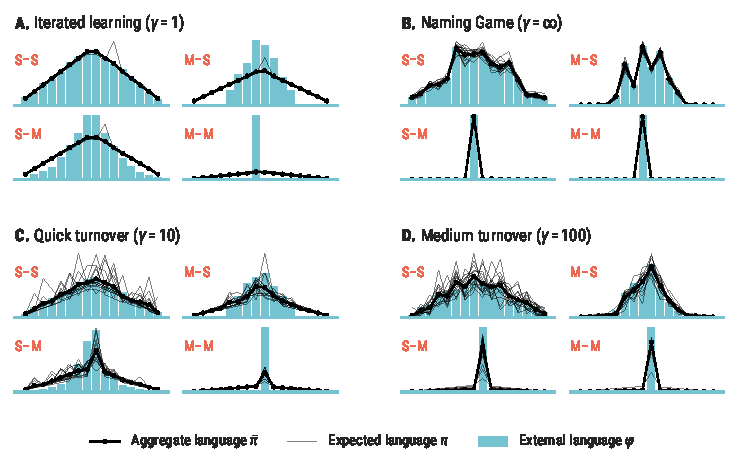
\includegraphics[trim=0.2cm 0 0 \figtopmargin]{FIG08-BNG-overview}
	
	\caption{%
	Typical outcomes of the Dirichlet-Categorical language name for the extreme strategies 
	(sample--sample, \textsc{map}--sample, sample--\textsc{map}, \textsc{map--map}) in populations with 
	immediate turnover (\textsc{a}, iterated learning, $\gamma=1$), 
	no turnover (\textsc{b}, naming game, $\gamma=\infty$) 
	and two intermediate turnovers (\textsc{c} and \textsc{d}).
	\figdetails{\figid{fig08} 
	$K = 16$, $N = 15$, $b = 1$, $T=10 000$}
	\label{fig:ch7:FIG08-bng-overview}}
\end{SCfigure}
%- - - - - - - - 





The eight extreme cases, with $\eta, \zeta, \gamma \in \{1, \infty\}$ are of special interest. 
With $\gamma=1$ the language game reduces to iterated learning, and with $\gamma=\infty$ it reduces to a naming game.
The pure sampling strategy (sample--sample) corresponds to $\eta=\zeta=1$; the mixed sampling-maximising strategies to $\eta=1, \zeta= \infty$ (sample--\textsc{map}) and $\eta=\infty, \zeta=1$ (\textsc{map}--sample); and the pure maximising strategy to $\eta=\zeta=\infty$ (\textsc{map--map}).
A systematic search through the space suggested that the behaviour of the game would relatively smoothly change between these eight extreme cases.
Characterising their behaviour therefore goes a long way to charting the behaviour one can expect from agent-based language models.
The result of cultural evolution in the extreme cases (and two intermediate population turnover rates) are shown again in figure \ref{fig:ch7:FIG08-bng-overview}.
The main conclusions it suggests are:
\begin{itemize}
	\item Bayesian naming games results in languages reflecting the bias, but shaped by cultural evolution.
	\item In iterated learning models, no agent faithfully represents the external language.
	\item Pure sampling strategies stay close to the bias, either perfectly (iterated learning), or imperfectly (naming game)
	\item Mixed strategies differently ‘exaggerate’ the bias: maximising languages results in some kind of pruning, maximising productions in some kind of exponentiation.
	\item Pure maximising strategies result in degenerate languages.
	\item The language spoken in an iterated learning model seems predictably determined by the biases — even for maximising strategies.
	\item Intermediate life expectancies interpolate between these two extremes.\footnote{%
		%>>>
		With one notable exception: there might be stable language change in between, but possibly only for a very limited parameter range.
		%<<<
		}
\end{itemize}
That, in short, that was the answer this thesis formulated on the first subquestion addressed in this thesis: what kind of behaviour can we expect from agent-based models of language evolution? Well, see figure \ref{fig:ch7:FIG08-bng-overview}, and interpolate!




\paragraph{empirical validity}

That might be a good start, but what does it tell us about language evolution?
In all fairness, I do not think I have formulated anything close to a clear answer to this question.
Perhaps because this is a not exactly an easy question.




In the second part of the thesis I identified numeral systems as an interesting test case for models of language evolution.
I gave various reasons, pertaining to the amount of linguistic data available, the sheer size of the design space (which makes for an interesting search problem), the balance between expressivity and simplicity in numerals and, most importantly, that the structure of numerals themselves suggest a reconstruction of their origins.
The last chapter tried to connect that reconstruction to agent-based models of language evolution.
That led to some interesting findings, such as the fact that the biases of agents and the constraints of the domain interact in different ways.
Or the sensitivity of naming games to subtle frequency biases in the underlying domain.




In fact, that finding is perfectly illustrative of the problem: all agents seem to be doing in these models is a more or less sophisticated form of frequency administration. 
Administration surely helped the rise of human civilisation, but perhaps not this kind of administration.
\emph{Perhaps}. 
The point is that adapting to  frequencies describes a \emph{mechanism} that amounts to an explanation of the observed phenomenon — but is it the right one, is it justified? 
Frequency ‘administration’ could explain the standardisation of bases, as we have seen in the last chapter.
But one could also explain that by using arguments of communicative efficiency, as \textcite{Hurford1987} also proposed.
Which one to prefer?
Or take a different example: the idea that compositionality emerged because it balances expressivity and compressibility.
The explanations suggested for one of the purest compositional structures, that of numerals, point in a quite different direction: a counting practice, grouping objects, or, later, processes of grammaticalisation.
Which one is it?



As soon as one leaves the world of models and enters the world of language, in this case numeral systems, it becomes clear that you have moved to a different, lower level of description.
One could conclude that the higher level description is ‘wrong’, but that would be too simple.
Descriptions at different levels are rarely perfectly aligned — that’s the whole point of having different levels of descriptions in the first place.
But what, then, is the conclusion?
Perhaps that it is time to see if the levels of description align at all.
That is, to see if the models can explain actual linguistic data, outside the computer or the lab.





\bigbreak\noindent
I did not like Berwick and Chomsky’s paper, as the reader could no doubt tell from the introduction.
Just as pretty much any other field of science, the ‘Kirby-type work’ has problems and good, sharp critiques are refreshing.
But the style — demeaning, territorial, grotesque. 
I mean, the academic equivalences thereof.
Science, the knowledge commons, those are, in the end, beautiful, praiseworthy things and you would hope for a more more communal spirit.\footnote{%
	%>>>
	Ah, how could I have missed that? 
	The second sense: “(of conflict) between different communities, especially those having different religions or ethnic origins: violent communal riots.”
	That explains everything.
	%<<<
}
In any case, there is one point at which I could not disagree with \textcite{Berwick2017}: when they write that, as far as they know, the “whisper down the lane” properties (slang for ‘iterated learning’) have not been applied to “the empirical phenomena of language change that linguists have actually measured” outside the lab or simulations. 
%Not as far as I know, either. 
It is just that I would prefer not to read that as a fatal blow, but as a programme.


\bigbreak\noindent
I will leave it at that. 
The remainder of this chapter lists the main contributions, some points of discussion and future work. 


\section{Main contributions}


The main two contributions of this thesis are (1) the Bayesian Naming Game, an attempt at unifying the naming game with the Bayesian model of iterated learning, and (2) the identification of numeral systems as a testbed for models of cultural language evolution. 
Various other additions to existing literature have been made throughout the thesis. The ones I believe to be of most interest are listed below.

\begin{itemize}		
	\item \textbf{Lineage-specific languages can reflect a prior.} 
		A demonstration that longer lifespans can lead to lineage-specific, shared languages that reflect the prior, but do not mirror it exactly. This suggests that cultural evolution \emph{can} change languages in nontrivial ways, while still being subject to innate constrains.
	
			
	\item \textbf{Random walks as a transmission model.}
		A new model of cultural transmission in the form of a random walk through a population of fixed size. 
		This combines the transmission chains with homogeneous mixing.

	\item \textbf{Connecting naming games to iterated learning}
	The thesis tried to connect two agent based modelling paradigm. Most specifically this results in a direct mathematical parallel between the model of \textcite{DeVylder2006} and Bayesian iterated learning models. 
	
	\item \textbf{Numerals as a testbed for language evolution.} 
		I have argued that numeral systems are a promising test case to relate models of language evolution with actual language.
		Numeral systems (i) allow one to model a subsystem of natural language directly; (ii) there is plenty of linguistic variation (i.e.\ the search of possible systems); (iii) the cognitive capacity for numerosity has been studied extensively; and (iv) there are benchmarks in the form of a reasonable reconstruction of the origins of numeral systems, which is moreover supplemented by recent empirical studies.
		
	\item \textbf{Realistic population turnover using Weibull distributions.}
		Proposed a more realistic death-process for iterated learning models based on the Weibull distribution, often used to model life-expectancy.
		Earlier iterated learning studies have often assumed constant hazard rates, which are unrealistic.
		
	\item \textbf{Revisited Hurford’s base games.}
		I have shown that Hurfords early simulations of the standardisation of a base are variants of the Naming Game.
		
	\item \textbf{Domain-adaptivity in the Base Game.}
		Demonstrated that the Base Game adapts to the domain in the sense that the behaviour depends on frequency patterns determined by domain.
		
	\item \textbf{Counting Game.}
		A new type of naming game in which agents negotiate a counting sequence.
		In this model simple numerals derive their meaning solely from their position in the sequence.
		
	\item \textbf{Packing strategy without grammar.}
		A reformulation of the packing strategy independent of the phrase-structure grammar proposed in \textcite{Hurford1975} in terms of the semantic (arithmetic) structure of the numerals.
		This is particularly relevant for empirical studies of this proposed universal.
\end{itemize}



\section{Future work}

Throughout this thesis, possibilities for future work have been identified.
Let me list the most practical points first, and then move on to the more interesting questions.

%...
\begin{itemize}
	\item \textbf{Other lateral inhibition strategies.}
	This thesis only compared Bayesian updating has only to the \emph{basic} lateral inhibition strategy in \textcite{Wellens2012}. 
	Wellens also mentions the so-called \emph{interpolated} \textsc{li} strategy, which can be interpreted as the Rescorla-Wagner or Widrow-Hoff rule. 
	In hindsight, that seems closer to Bayesian updating (in form, at least) and future work could address the exact relation.

	\item \textbf{Measures for the Bayesian naming game}.
	\label{fw:measures-bng}
	The measures used to analyse the Bayesian naming game could be improved by developing appropriate variants of measures used in naming games (communicative success, number of (unique)). 
	The methodology of chapter \ref{ch:counting-games} could be a starting point.
	
	\item \textbf{Scaling relations.}
	The change in convergence time in the Bayesian naming game under varying population, vocabulary and bottleneck size could be investigated more thoroughly, either empirically or analytically.
	
	\item \textbf{Models of life-expectancy.}
	Chapter \ref{ch:bayesian-naming-games} argued for more realistic models of life-expectancy without actually analysing whether they make a difference in the simulations. 
	A systematic analysis would be valuable.
	
	\item \textbf{Random walks vs.~homogeneous mixing.}
	Preliminary experiments did not reveal any systematic differences between random walks and homogeneous mixing in the Bayesian naming game, but this should be checked in a principled fashion.
	
	\item \textbf{Mathematical problems.}
	The mathematical analyses gave rise to several problems.
	The first concerns the characterisation of the posterior distribution of an agent with a maximising word strategy $\zeta > 1$; see appendix \ref{app:bng}.
	Another concerns the bias in Hurford’s additive base game: has this distribution (proportional to the difference of two harmonic numbers) been studied before?
\end{itemize}
%...

\paragraph{Other Bayesian naming games}

This thesis mainly developed the Dirichlet-categorical naming game as the simplest instantiation of a more general framework.
Future work could study other models inside the same framework.
An interesting possibility would be to drop the conjugacy assumption, and consider more general probabilistic models.
In fact, the Dirichlet-categorical model surfaced from early experiments with Bayesian agents represented as so called \emph{probabilistic programs}.
Probabilistic programming (see \cite{Ghahramani2015} for an overview) provides a remarkable representational flexibility by using programming languages to specify the models, and their universal approximate inference algorithms (sampling or variational methods) significantly speed up development time.
The downside in our context would be that poor inference could have unexpected results when repeated for tens of thousands of rounds and thus trouble the analyses.


\paragraph{Connections to biological evolution}

\textcite{Reali2010} were the first to connect Bayesian models of iterated learning to biological evolution, i.e.\ the Wright-Fisher model. 
Since the Bayesian Naming Game is in many ways identical to their model, it seems worthwhile to explore further connections with models developed in population genetics. 




\paragraph{Nonparametric extension of the Bayesian Naming Game}

The Bayesian Naming Game made the simplifying assumption that the number of words in the population is fixed, an assumption made earlier in \textcite{DeVylder2006}.
The model would stay closer to the original naming games if this assumption could be dropped.
Invention after all plays a crucial role in the Naming Game \parencite{Steels2011}, but more generally it has been argued that inventors play an important role in language change and evolution \parencite{Hurford1987}.
Fortunately, there is a straightforward extension of the Bayesian Naming Game which does not fix the number of categories — is not \emph{parametric} in that sense.
This model would use an infinite analogue of the Dirichlet distribution, a Chinese restaurant process, that allows for the use of an arbitrary number of words.
Every agent then faces the choice of either using an old word or inventing a new one.
This extension has been discussed in the iterated learning literature before  \textcite{Reali2010,Burkett2010}.




Combined with population turnover, the non-parametric model seems to solve another issue: that words never disappear from the population completely.
In classical lateral inhibition games, words scoring below a certain threshold are removed.
This mechanism allows the emergence of \emph{efficient} vocabularies.
Population turnover could replace that mechanism in a non-parametric variant of the Naming Game: low-frequency words might simply not be acquired by newborn agents, and consequently die out.
If this prediction is indeed true, it suggests a very exciting possibility.
Suppose one splits the population in two parts at a certain point in time, and let both halves continue the game separately.
Given the stochasticity of the game, it seems likely that different words would die out, effectively leading to different lineages.
%As discussed in chapter ??, strong lineage-specific trends have indeed been reported \parencite{Dunn2011} and 
Future work could investigate such ‘linguistic speciation’ in a non-parametric extension of the Bayesian Naming Game.





Note that this also highlights a problem with the notion of ‘lineage specificity’ as I have used it.
‘Lineages’ were understood to mean ‘runs’, since it has not been shown that one can, say, split the population and develop two distinct branches.
For the Bayesian naming game, the later seems moreover unlikely, since the language develops its characteristic shape primarily in the early phase of the game, before agents reach ‘adulthood’.
After that, the population only converges to a completely stable language, which is not realistic either \parencite{Kirby2001}.
Increasing population turnover addresses this, and the nonparametric suggestion outlined above might solve the former.





\paragraph{Mathematical analysis of the Bayesian Naming Game}

Simulations indicate that coherence emerges in the Bayesian Naming Game, but I have not provided a formal proof of this.
In fact, there are two separate questions: (i) do all agents converge to the same distribution? 
And (ii) can one characterise this distribution in terms of the parameters $\eta, \zeta$ and $\gamma$?
It seems unlikely that this is a simple problem, since even the special case of the naming game has so far resisted analytical scrutiny (\textcite{DeVylder2006} only provide analytical results for a deterministic variant of the game).
One possible line of attack would investigate whether the limiting distribution is indeed a sample from some distribution around the prior.
If so, a characterization of that distribution would be likely to provide valuable further insights into many models of cultural language evolution simultaneously.


\bigbreak\noindent
And the list continues. 
But that’s it for now.




\end{document}
Of course, this thesis has not characterised all agent-based models of cultural language evolution — far from it.
Small variations in the script result in different games (e.g.~counting games, or see \cite{Baronchelli2007}) that need not lie in the space of agent based models captured by the Bayesian language game.
In some cases this results in substantially different behaviour \parencite{Baronchelli2007}, in other cases the long-term behaviour is essentially unchanged (e.g.\ the counting games).
A certain robustness in this respect seems desirable.
If, after all, a small change can radically alter the outcome of the model, one wonders to what extent it is even feasible to approach the cultural evolution of language through models.



This thesis set out to address two questions: first, what kind of behaviour can we expect from agent-based models of language evolution? and second, how does that behaviour relate to actual evolved language?
The first three chapters addressed the first question, by first looking at the iterated learning tradition, then at naming games, and finally proposing a unified view on both in the form of the Bayesian naming game.
Iterated learning \parencite{Kirby2001,Brighton2002,Smith2002} developed the idea that cultural transmission is the shaping force in language.
It forces language to by becoming better transmissible.
Computer simulations of the emergence of compositional structure were argued to demonstrate the validity of this theory.
The problem, however, was that the generalisation algorithms implicitly introduced various biases, perhaps pressuring towards compositional languages.
The Bayesian models of iterated learning \parencite{Griffiths2007a} addressed this problem by explicitly specifying the inductive biases of the agents in the form of a prior.
This moreover characterised the long-term behaviour. 
The transmission chains were essentially Markov chains that, when ergodic, would keep revisiting the entire state space of languages.
Over time, the probability that an agent would be in any particular state, i.e., would use a particular language, was given by the prior distribution.
This \emph{convergence to the prior} was however shown to break down in more complicated population structures and resulted in a rather [...]


Reaching language stability goes to the heart of naming games.
These games study how a population without central coordination can negotiate a shared vocabulary.
For that to happen agents have to align their vocabularies after every interaction, which they can do using various strategies.
All the strategies we discussed had the same effect insofar the population reached coherence and thus learned to communicate effectively.
That this \emph{should} happen is corroborated by the convergence proof of \textcite{DeVylder2006}, although it only applied to a deterministic, aggregate variant of the naming game.




Although the interaction between the two communities is extremely limited, their models are not so far apart.
Chapter \ref{ch:bayesian-naming game} introduced the \emph{Bayesian naming game}, with the \emph{Dirichlet-categorical naming game} as a specific instantiation.
It adopted the Bayesian methodology from iterated learning, while generalising the model of \textcite{DeVylder2006}.
The resulting behaviour of the \textsc{dc} naming addressed many of the shortcomings identified in the earlier chapter.
Most importantly, the population converges to a shared language that reflects the learners biases, but not transparently. 
The convergence to the prior is thus replaced by a reflection of the biases.
Stable languages were also obtained, that exhibited the nontrivial effects of the cultural process.


Changing the population structure of the Bayesian naming game led to the Bayesian language game.
This game performs a random walk through the population, and assigns agents a certain life expectancy $\gamma$.
With a very small life expectancy (1 interaction), it reduces to an iterated learning game, but with a long life-expectancy, it becomes a naming game.
The parameter $\gamma$ interpolated between the two agent-based paradigms, and allowed us to characterise the behaviour of the most important agent-based models of language evolution.
Mixed sampling-maximising strategies exaggerate innate biases, pure sampling strategies reflect the biases more directly and pure maximising strategies result in degenerate languages.
The life expectancy determines how faithful this ‘reflection’ is.
With iterated learning models, the \emph{external} language, the utterances faithfully reflects the (exaggerated) bias.
With naming games, there is room for lineage specific cultural variation around the bias.




All this had left one important point unaddressed: how realistic are these models when compared with actual language?
The second part of the thesis addressed that.
The first thing to do was arguing for a convincing test case, which was found in numeral systems.
Numeral systems seem ideally suited because they balance expressivity and compressibility near-perfectly.
Iterated learning has earlier been argued to produce exactly those kind of structures \parencite{Kirby2015}.
Moreover, there is a wealth of empirical data about numeral systems, illustrating the vast design space they lie in. 
Nevertheless, languages have settled on systems in a relatively small part of the space, and models of cultural evolution could try to explain why so.
Their explanations can be directly tested against a fairly well-supported account of the actual historical development of numeral systems — a rarity, in language.
%todo cognitive constraints?


To connect all the dots, the last chapter made a first start with modelling the emergence of numeral systems.
Some pioneering work had already been done in this direction by James Hurford, in the form of two base games.
Reanalysing the games revealed that they were essentially naming games with certain specific implicit biases.
Crucially, these biases resulted from hard constraints, which sets them apart from the biases in the Bayesian naming game.
% todo








%todo mixed/pure, 
%todo in ch on il: mention that Griffiths&K argue that ergodicity is a realistic  assumption



